% !TEX root = report.tex
\section{Results / Analysis}
We recognize that the Java and C++ queue delegation implementations will have inherent performance differences. The purpose of the analysis in this section is to determine a baseline performance difference between MonitorT (Java) and QD Lock (C++), where neither have elimination. Then, we analyze the performance difference by adding elimination to the QD Lock version (i.e., QD Elimination Lock).

Figure~\ref{fig:baseline} shows the baseline performance comparison between MonitorT and QD Lock (neither having stack elimination). Figure~\ref{fig:fig00} shows that the two implementations are relatively similar, with the C++ implementation slightly outperforming MonitorT, as would be expected. It is interesting to note that they both seem to scale equally well with increasing thread counts. However, Figure~\ref{fig:fig01} shows that their performance is relatively volatile when the delegation queue size varies. As the queue size increases, both implementations have longer run times.

\begin{figure}[]
\centering
\subfloat[][]{\label{fig:fig00}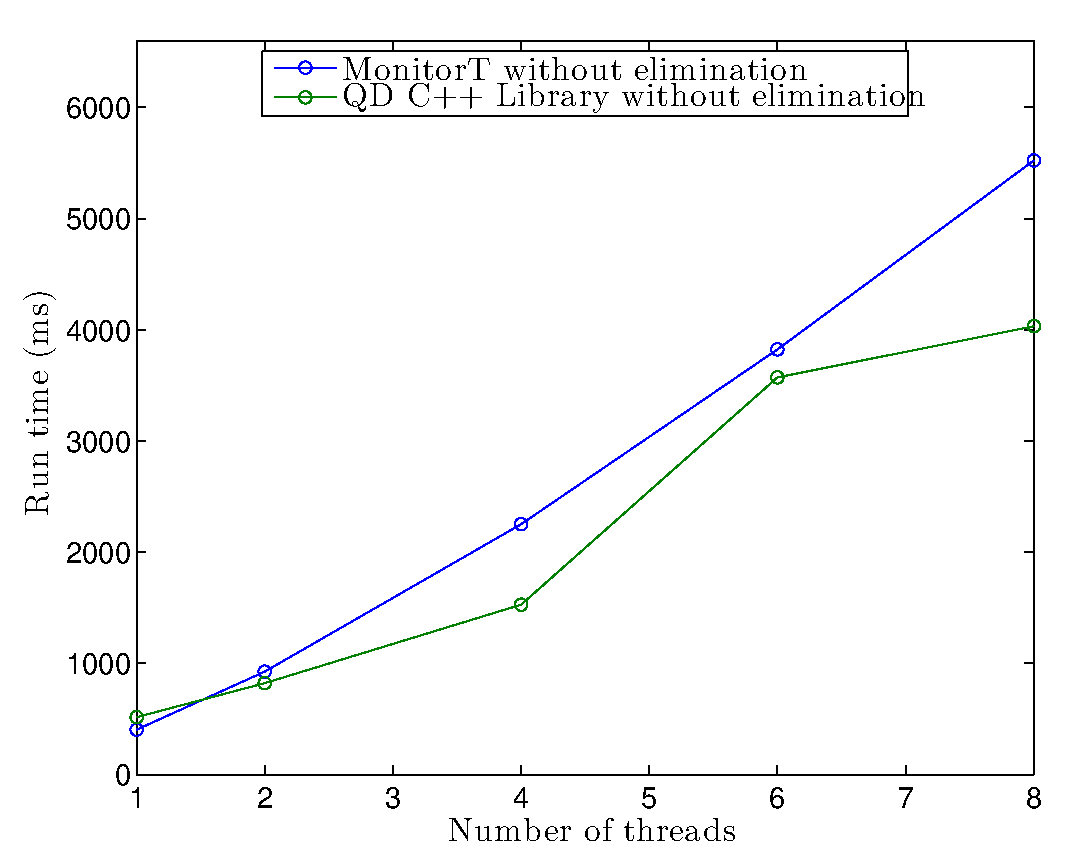
\includegraphics[width=.49\textwidth]{figs/00_TimeVsThreads_cppNoElim_javaNoElim.eps}}
\subfloat[][]{\label{fig:fig01}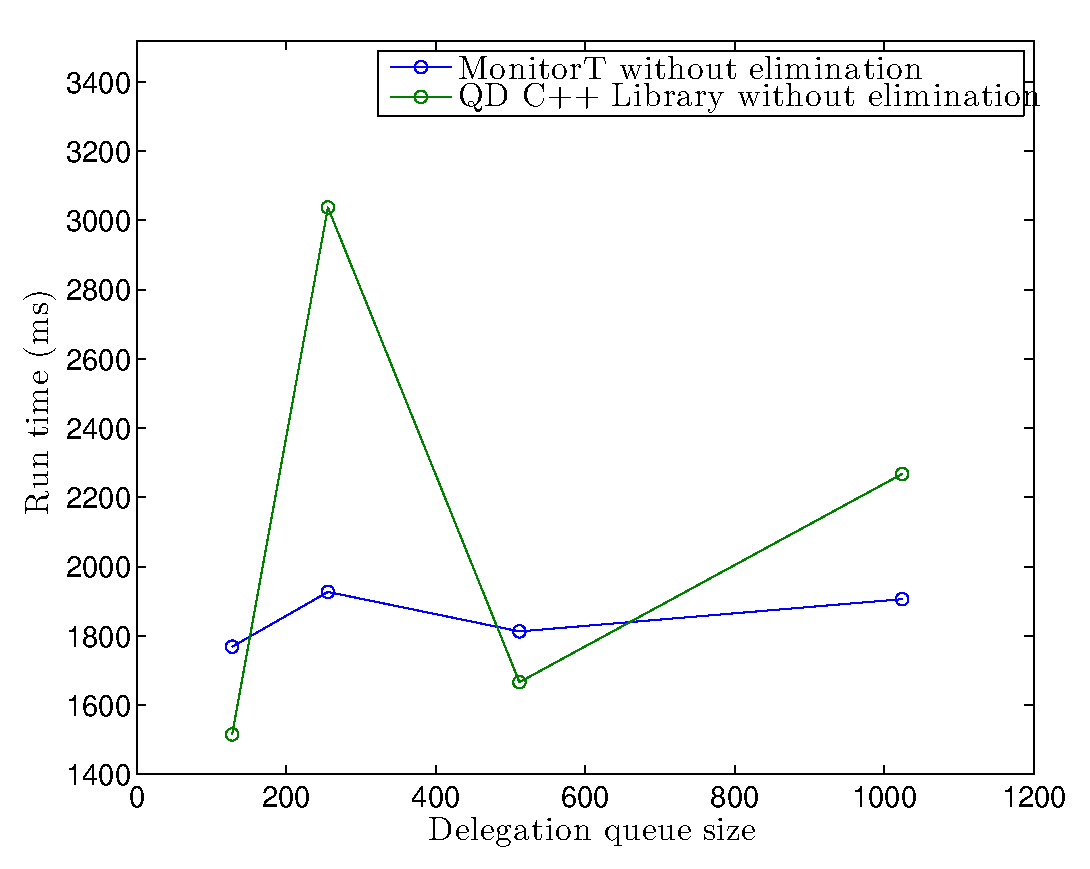
\includegraphics[width=.49\textwidth]{figs/01_TimeVsQDsize_cppNoElim_javaNoElim.eps}}\\
\caption[]{Baseline comparison of the MonitorT implementation (Java) and the QD Lock (C++): \subref{fig:fig00} varying the number of threads, and without elimination for either implementation (queue size = 256, push ratio = 0.5); \subref{fig:fig01} varying the delegation queue size, and without elimination for either implementation (threads = 4, push ratio = 0.5).}
\label{fig:baseline}
\end{figure}

%======================================================================

In Figure~\ref{fig:fig02}, we see that the performance of QD Elimination Lock is better than QD Lock in Figure~\ref{fig:fig00}, as expected. The performance benefits are greater at higher thread counts.

\begin{figure}[!h]
\centering
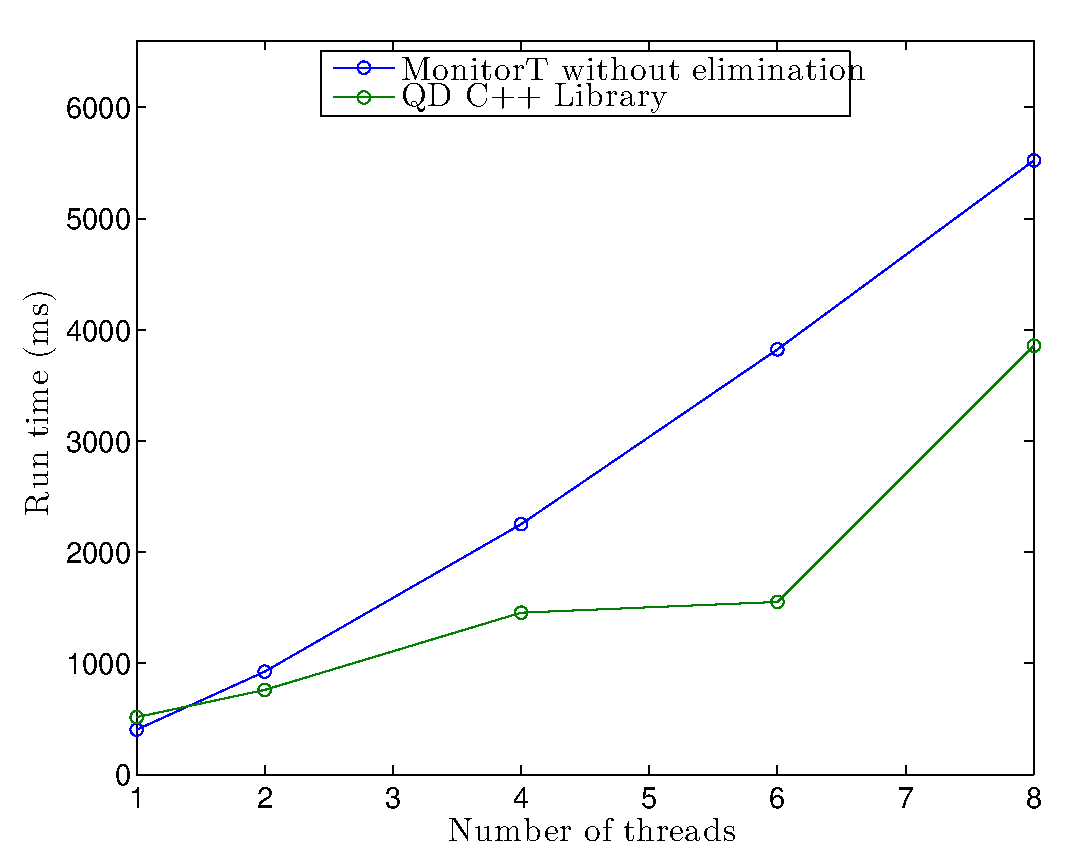
\includegraphics[width=.75\textwidth]{figs/02_TimeVsThreads_cppElim_javaNoElim.eps}
\caption[]{Comparison of the MonitorT implementation (Java) and the QD Elimination Lock (C++), varying the number of threads (elimination included for C++ implementation, not for Java). Queue size = 256, elimination array size = 4, push ratio = 0.5.}
\label{fig:fig02}
\end{figure}

%======================================================================

Figure~\ref{fig:qdlock} shows that QD Elimination Lock consistently outperforms QD Lock, across sweeps of all parameters. As the number of threads increases, the speedup of QD Elimination Lock over QD Lock increases. Figure~\ref{fig:fig04} shows that the elimination array size should not be to small nor too large, as this yields either too much contention (show where array size = 2) or not enough matches between pushes and pops (shown where array size = 16).

As the delegation queue size increases, the delegate thread spends more time executing the other threads' workloads, eventually slowing the execution of the delegate thread's own work. This is seen in Figure~\ref{fig:fig05}, for both the QD Lock and QD Elimination Lock. This behavior would not be expected in MonitorT, since MonitorT uses a separate thread for the delegation queue.

We see in Figure~\ref{fig:fig06} that as the push percentage increases, we would have expected the performance to decrease since there would be fewer matches between pushes and pops. But instead we see that the performance either increases or remains steady. Another anomaly is that we would expect QD Lock to have flat performance across all push percentages, since it views all operations alike.

\begin{figure}[]
\centering
\subfloat[][]{\label{fig:fig03}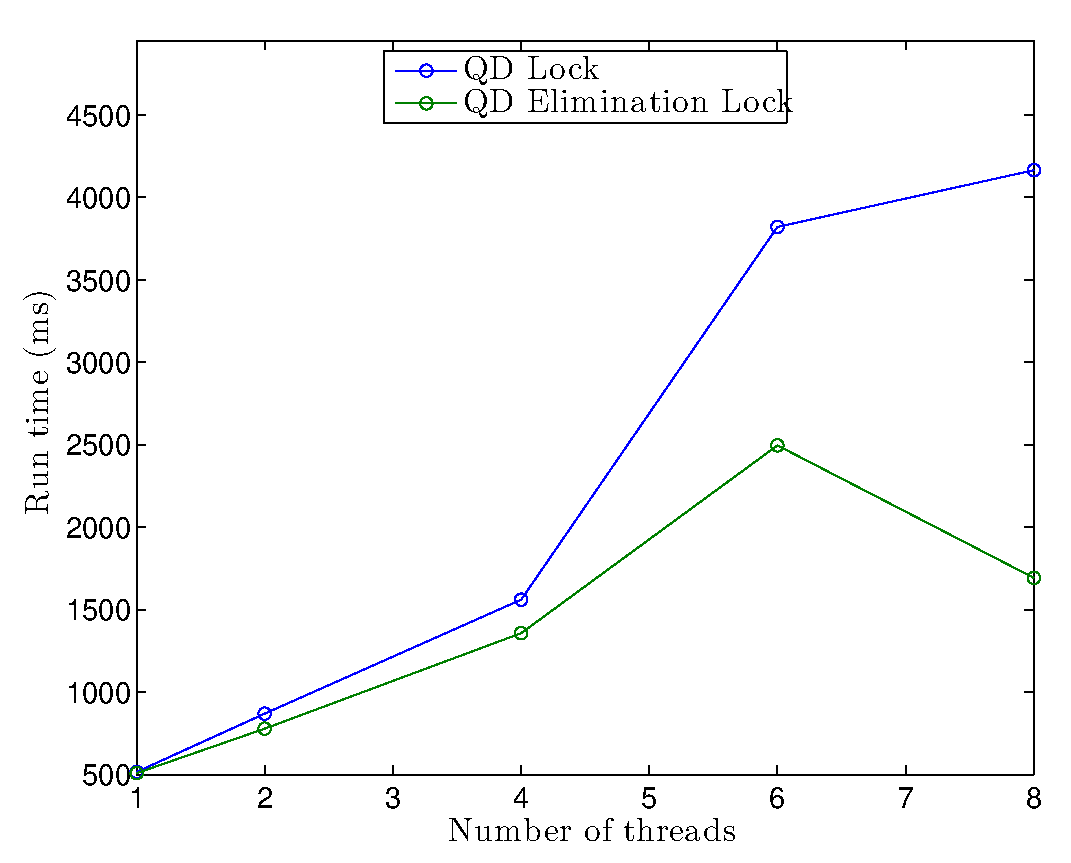
\includegraphics[width=.49\textwidth]{figs/03_TimeVsThreads_cppElim_cppNoElim.eps}}
\subfloat[][]{\label{fig:fig04}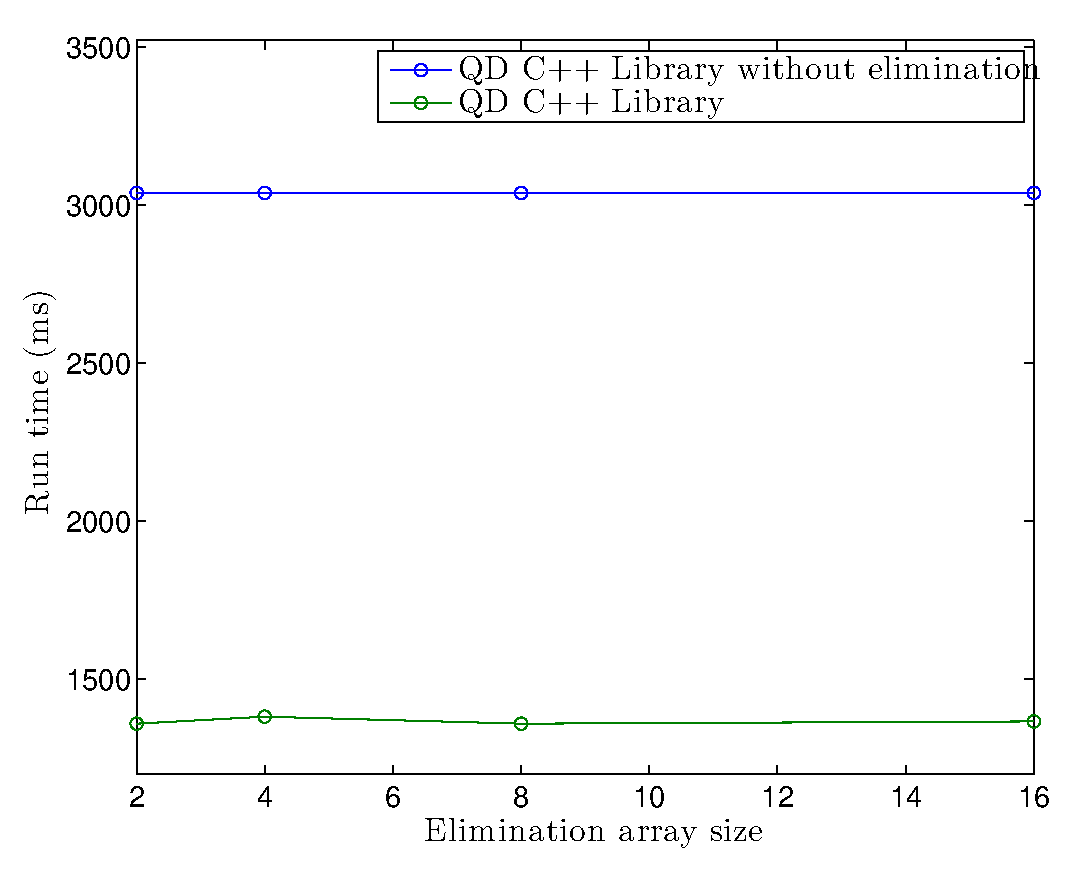
\includegraphics[width=.49\textwidth]{figs/04_TimeVsElsize_cppElim_cppNoElim.eps}}\\
\subfloat[][]{\label{fig:fig05}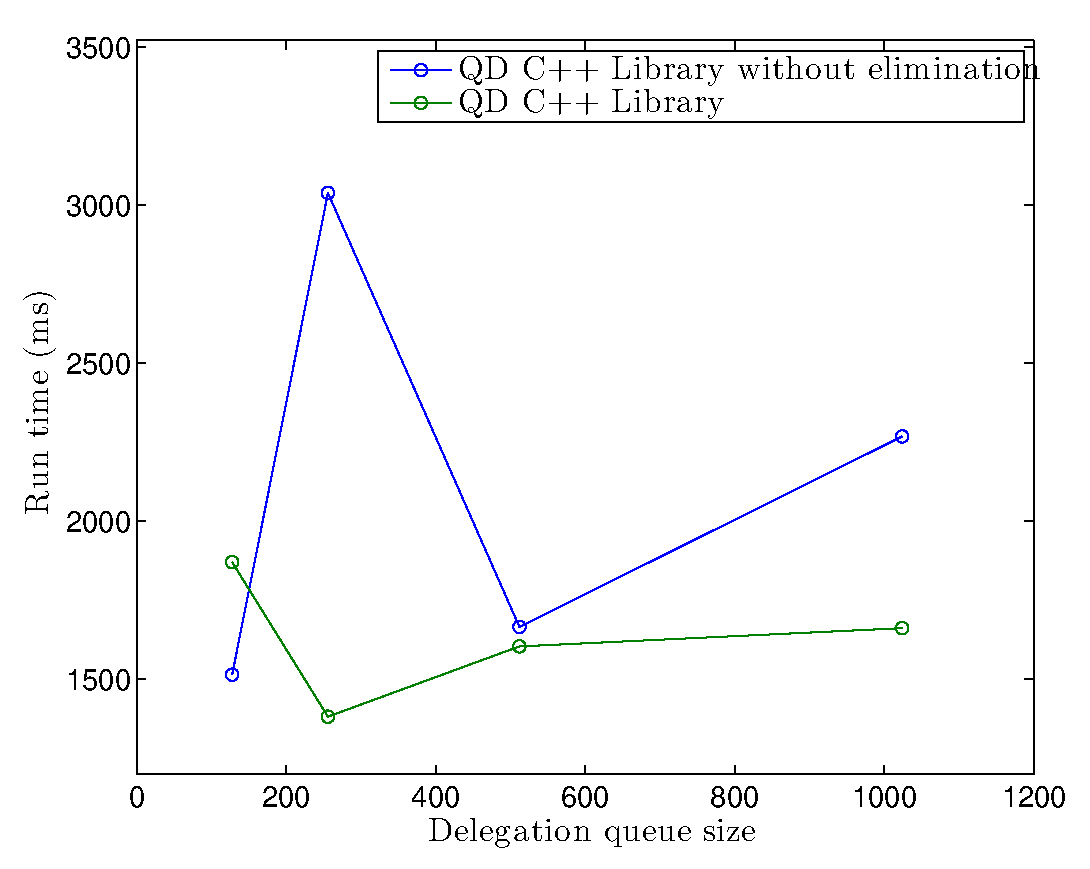
\includegraphics[width=.49\textwidth]{figs/05_TimeVsQDsize_cppElim_cppNoElim.eps}}
\subfloat[][]{\label{fig:fig06}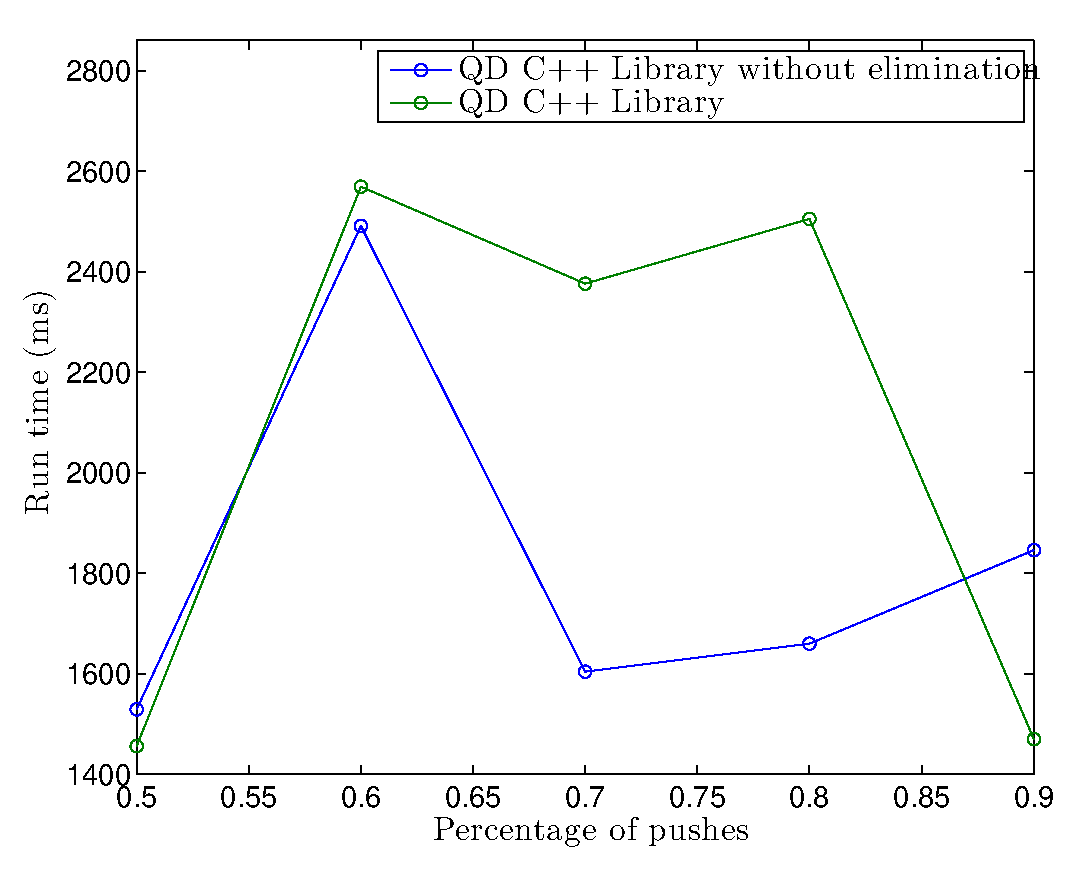
\includegraphics[width=.49\textwidth]{figs/06_TimeVsPctPush_cppElim_cppNoElim.eps}}
\caption[]{QD Elimination Lock versus QD Lock (both C++), while varying each parameter separately: \subref{fig:fig03} varying the number of threads (elimination array size = 4, queue size = 256, push ratio = 0.5); \subref{fig:fig04} varying the elimination array size (threads = 4, queue size = 256, push ratio = 0.5); \subref{fig:fig05} varying the delegation queue size (threads = 4, elimination array size = 4,push ratio = 0.5); \subref{fig:fig06} varying the push ratio (threads = 4, elimination array size = 4, queue size = 256).}
\label{fig:qdlock}
\end{figure}

%======================================================================
The performance values observed in Figure~\ref{fig:thrd_and_elsize} also show the relationships between thread count, delegation queue size and elimination array size. Figures~\ref{fig:fig07a} --~\ref{fig:fig07d} represent changing the delegation queue size from 128 to 2048, respectively. The different queue sizes appear to have a negligible effect on the run time, except for the first case where the performance is better with a queue size of 128. These figures also show that the thread count had the largest effect and the elimination array size had minimal effect, since the multiple lines plotted for run time versus thread count exhibit minimal changes for the different elimination array sizes.

\begin{figure}[]
\centering
\subfloat[][]{\label{fig:fig07a}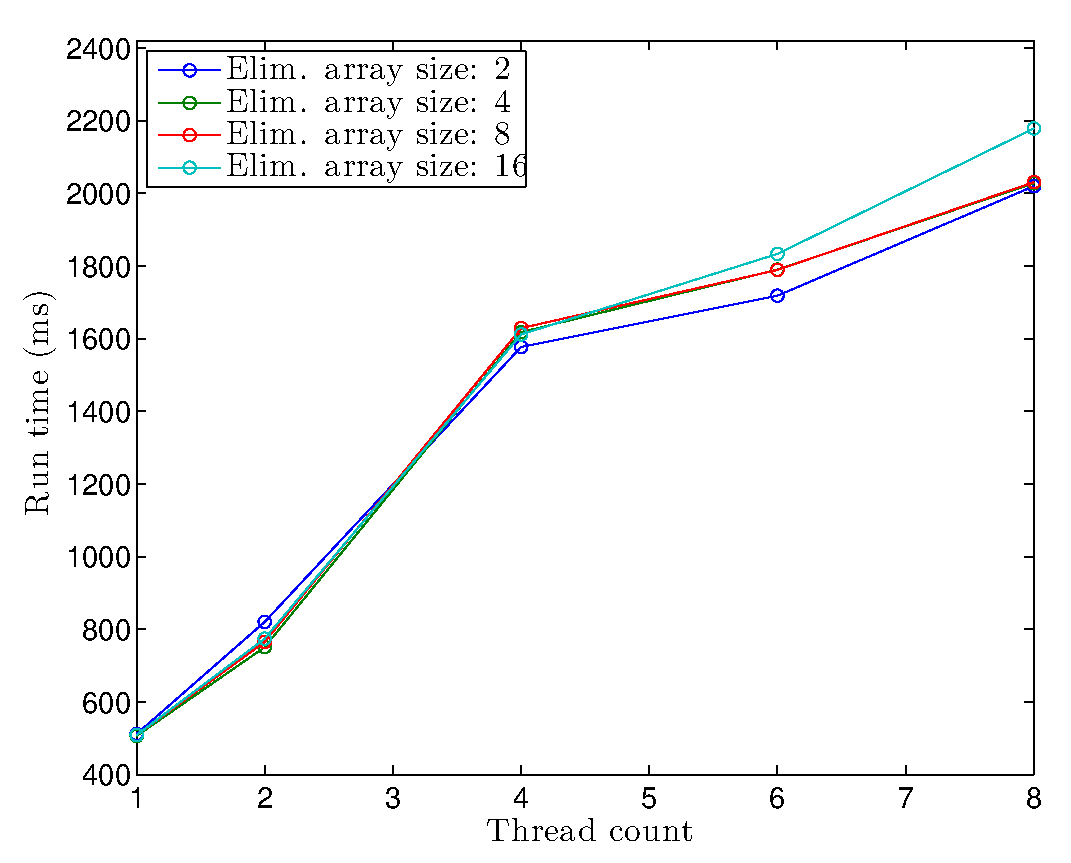
\includegraphics[width=.49\textwidth]{figs/07a_Q128_TimeVsThreadsVsEsize_cppElim.eps}}
\subfloat[][]{\label{fig:fig07b}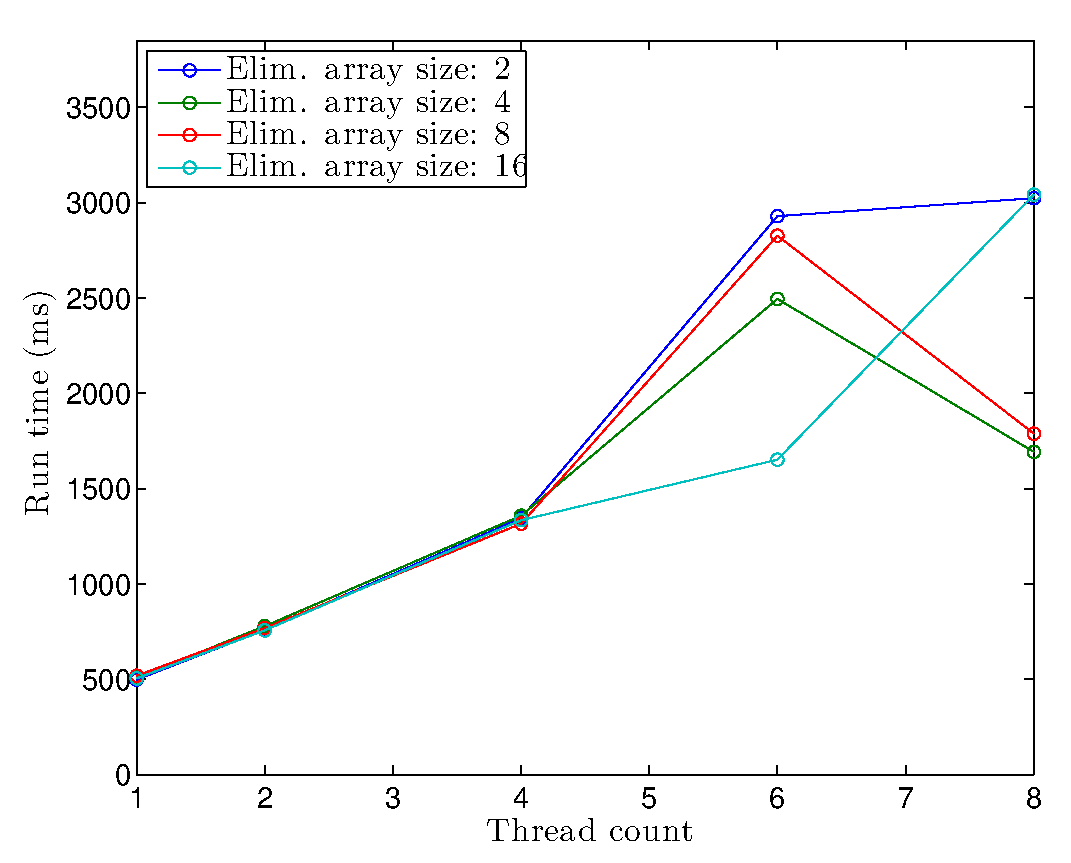
\includegraphics[width=.49\textwidth]{figs/07b_Q256_TimeVsThreadsVsEsize_cppElim.eps}}\\
\subfloat[][]{\label{fig:fig07c}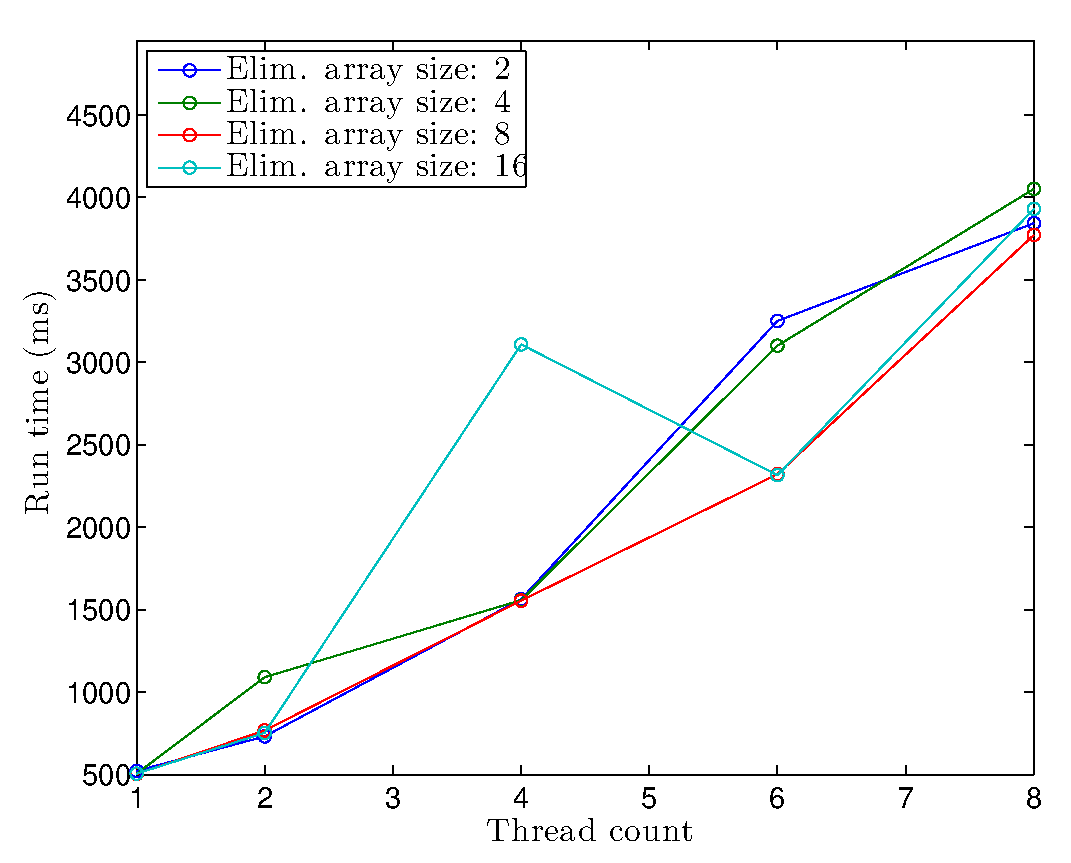
\includegraphics[width=.49\textwidth]{figs/07c_Q512_TimeVsThreadsVsEsize_cppElim.eps}}
\subfloat[][]{\label{fig:fig07d}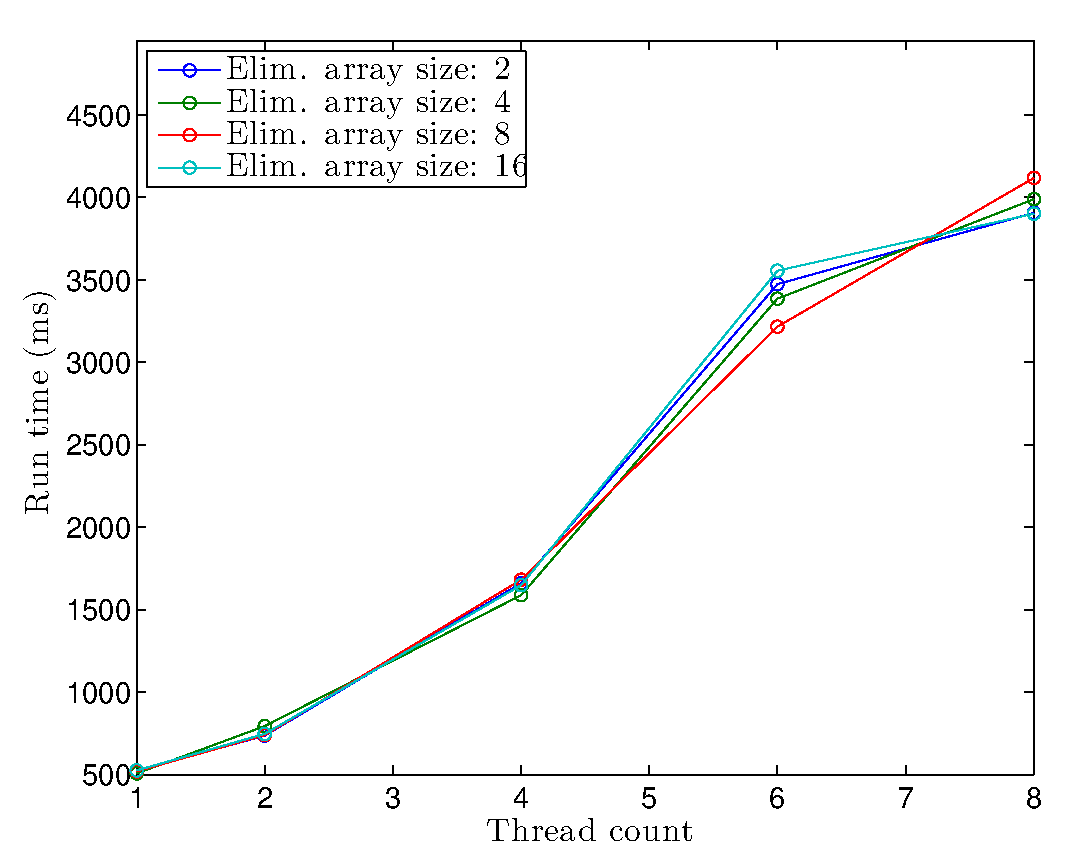
\includegraphics[width=.49\textwidth]{figs/07d_Q1024_TimeVsThreadsVsEsize_cppElim.eps}}
\caption[]{QD Elimination Lock performance versus thread count and elimination array size - each graph represents a different delegation queue size, while multiple elimination array sizes are plotted in each graph: \subref{fig:fig07a} queue size = 128; \subref{fig:fig07b} queue size = 256; \subref{fig:fig07c} queue size = 512; \subref{fig:fig07d} queue size = 1024. Push ratio = 0.5.}
\label{fig:thrd_and_elsize}
\end{figure}

%======================================================================
The elimination array size's minimal effect on performance is reflected again in Figure~\ref{fig:fig08b}, where the performance for each thread count remains relatively flat across all elimination array sizes. This plot also shows how increasing the number of threads monotonically decreases the performance, establishing the effects of contention at the higher thread counts.

Figure~\ref{fig:fig08a} shows that initially, increasing the delegation queue size adversely affects performance. However, for delegation queue sizes above 1024, the performance levels out.

\begin{figure}[]
\centering
\subfloat[][]{\label{fig:fig08b}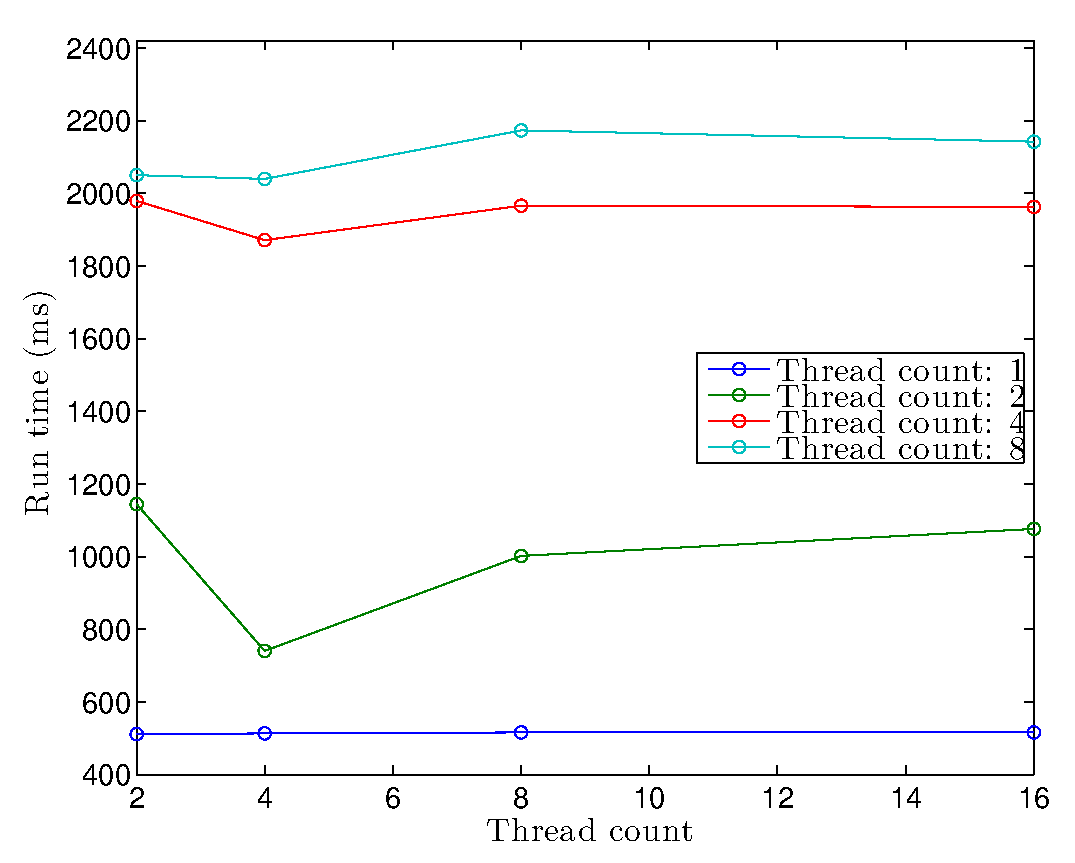
\includegraphics[width=.49\textwidth]{figs/08b_Q128_TimeVsEsizeVsThreads_cppElim.eps}}
\subfloat[][]{\label{fig:fig08a}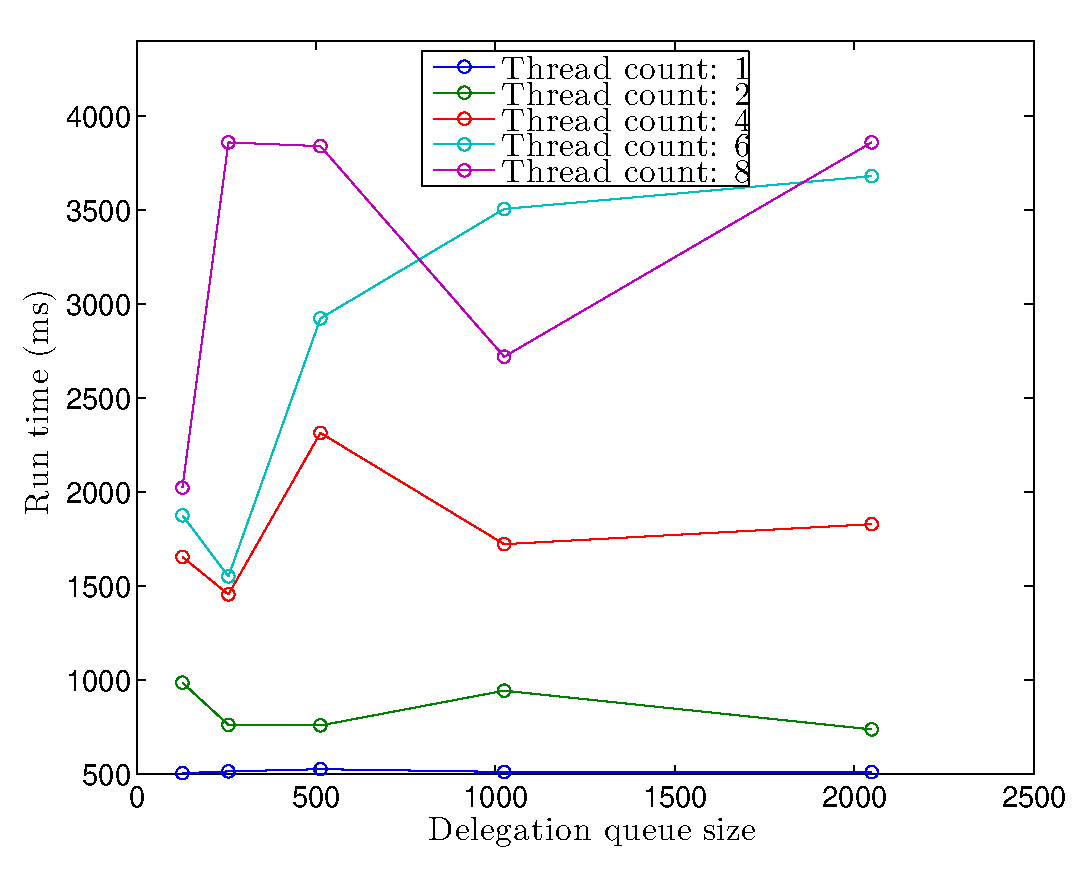
\includegraphics[width=.49\textwidth]{figs/08a_E4_TimeVsEsizeVsThreads_cppElim.eps}}
\caption[]{\subref{fig:fig08b} QD Elimination Lock performance versus elimination array size and thread count. Push ratio = 0.5. \subref{fig:fig08a} QD Elimination Lock performance versus delegation queue size and thread count.}
\label{fig:qdsize_and_thrd}
\end{figure}
